% !TeX root = ../../main.tex
\chapter{Design}
\label{chap:design}

\section{Analysing the Problem}
Problem Analysis was simple as I had clearly defined goals for the project. Making decisions for the project when you are your own product owner is significantly easier as you just have to satisfy your own goals with no risk of others having other views about where the project should go which could slow progress. Most of my analysis was done on a rolling basis, with me coming up with ideas over a period of a few weeks and noting them down for later use, then expanding on them when I got to working on that section of the project.

\section{Ensuring Ease of Use}
The app needs to be easy to use, if it isn't then the user may end up using other, less secure smart lock products. At the end of the day most users don't care about security, or at least they only care that the product claims to be secure. Most users just care about how easily they can setup and use the product. If they have problems whilst trying to do that then that's when you start to get bad reviews and unsatisfied users. To ensure ease of use, my approach will simply be to have as few obstacles as possible between the user and getting the lock ready to use.

\subsection{App User Interface}
The apps user interface will be very simple as it must be easy for an inexperienced user to understand and use. Overall, the app needs to be able to: let the user signup for an account or login to their existing account; setup their device if they don't have one already attached to their account; and lock or unlock the door. Anything on top of that will be added if time is available at the end of the project as the main focus is to prove that good security can be implemented and that if the system were to be extended it could be both secure and feature filled.

\section{Ensuring Security}
The security of the system will be ensured in many ways, most of which are analysed in the literature review. Here I will run over the security measures I will implement, and any further security measures that could be implemented given adequate time.

\subsection{TLS/HTTPS}
Ensuring that all communication is sent through HTTPS using at least TLS 1.2 will be a huge step towards having a secure system. TLS is the protocol used for any website that you would visit on your browser that is using HTTPS technology. There are a huge array of benefits received from using TLS such as: 
\begin{itemize}
	\item Encryption of all transferred data
	\item Encryption of metadata such as the endpoint you are connecting to
	\item Verification that the server you are talking to owns the domain you are connected to
	\item Protection against replay attacks
\end{itemize}
There are plenty of other benefits, those are just some of the most major ones. This will definitely be used in my project for all communication as it takes care of a lot of security concerns automatically.

\subsection{Certificate Pinning}
Certificate pinning is another very important but rarely used security measure. If you are connecting to a known server who's certificate doesn't change constantly, then you can ensure that you only connect to that server by pinning the certificate you connect to. In my case I will be using LetsEncrypt certificates which change every 3 months, so instead of pinning the main certificate I will pin the Certificate Authorities (CA) certificate. This is less secure, however it means that you are guaranteed to only connect to a system that has been issued a certificate by that CA for that domain, this is still a very high level of security as CA's are trusted to only issue certificates to the owner of the domain.

\subsection{CAA DNS Record}
Certificate Authority Authorization (CAA) DNS Records are there to ensure that only the Certificate Authority that you're using can issue certificates for your domain. When a CA is testing whether the request for a certificate is coming from the owner of the domain, one of the checks they do is to see if there is a CAA record on the DNS for the domain, and if so, whether they are listed as one of the authorised CA's. If they are not, they won't issue a certificate for the domain, therefore stopping any potential false certificates from being created if somehow an attacker managed to fool the system into believing they owned the domain. This will also definitely be used within my project as provides a lot of extra security for just a couple of seconds of setup.

\subsection{Central Server}
In my system I will be implementing a central server that will store accounts, registered devices, settings, device status, etc. This system will be the central trust point for the system as it will be considered secure at all times. Communication to and from the server will be secured as mentioned above using TLS/HTTPS and the server can be verified using certificate pinning along with the CAA DNS Record to ensure only LetsEncrypt can issue certificates for the smartlockapp.zackpollard.pro domain. The server will provide an API that the user and devices can connect to in order to talk to each other. This will be the main communication method between the smart lock and the users device, all unlock requests and other interactions will go through the server. If other authentication devices are implemented locally, then those will be able to communicate directly with the Core RPi in order to unlock the door, however that will be within the closed loop of the home network and will also all be encrypted using HTTPS/TLS. The central server will be a core part of the system so will definitely be used within the project.

\subsection{Offline Temporary Tokens}
This idea is for if/when the internet in the house goes down or the Core RPi just loses connection to the network. In that case, the core server would detect that the Core is no longer connected and would send a notification to the admin account for the lock. This notification would tell the user that they can download and distribute offline keys that the central server has pre-prepared with the lock for this occasion. These keys will allow the admin to control the lock even when the connection to the server has been lost, and the keys can also be shared with family and friends that may need access to the property during the time that the internet connection is down. Once the connection comes back up, these keys are immediately invalidated by the Core RPi and new keys are established between the central server and Core RPi for the next time that the internet connection becomes unavailable.

\subsection{Core UUID Changing}
The Core RPi will have a UUID that is generated during initial setup. This will be the main identifier for the device, there will be no master key or anything similar, just a UUID, device name, and the JWT that it uses to authenticate with the API on the central server. Every time the device is setup with another account, the UUID is changed although the device name remains the same. This changes the generated JWT even more as it will also incorporate a timestamp of the current time. This system completely eliminates the issues mentioned in the problem statement regarding the august locks ``firmware key.''

\section{User and Data Flow}
The flow of data around the system and the way in which the user will interact with the system to cause this data flow is important to get established early on as it is the basis around which the system will be built.

\subsection{Technical System Overview}
Figure 4.1 below shows the overview of how the seperate components of the system will communicate with eachother. This is the initial idea and so details could change slightly when programming begins however this is the main idea as to how it will all come together.

\begin{figure}[H]
	\caption{Block Diagram of the System Overview}
	\centering
		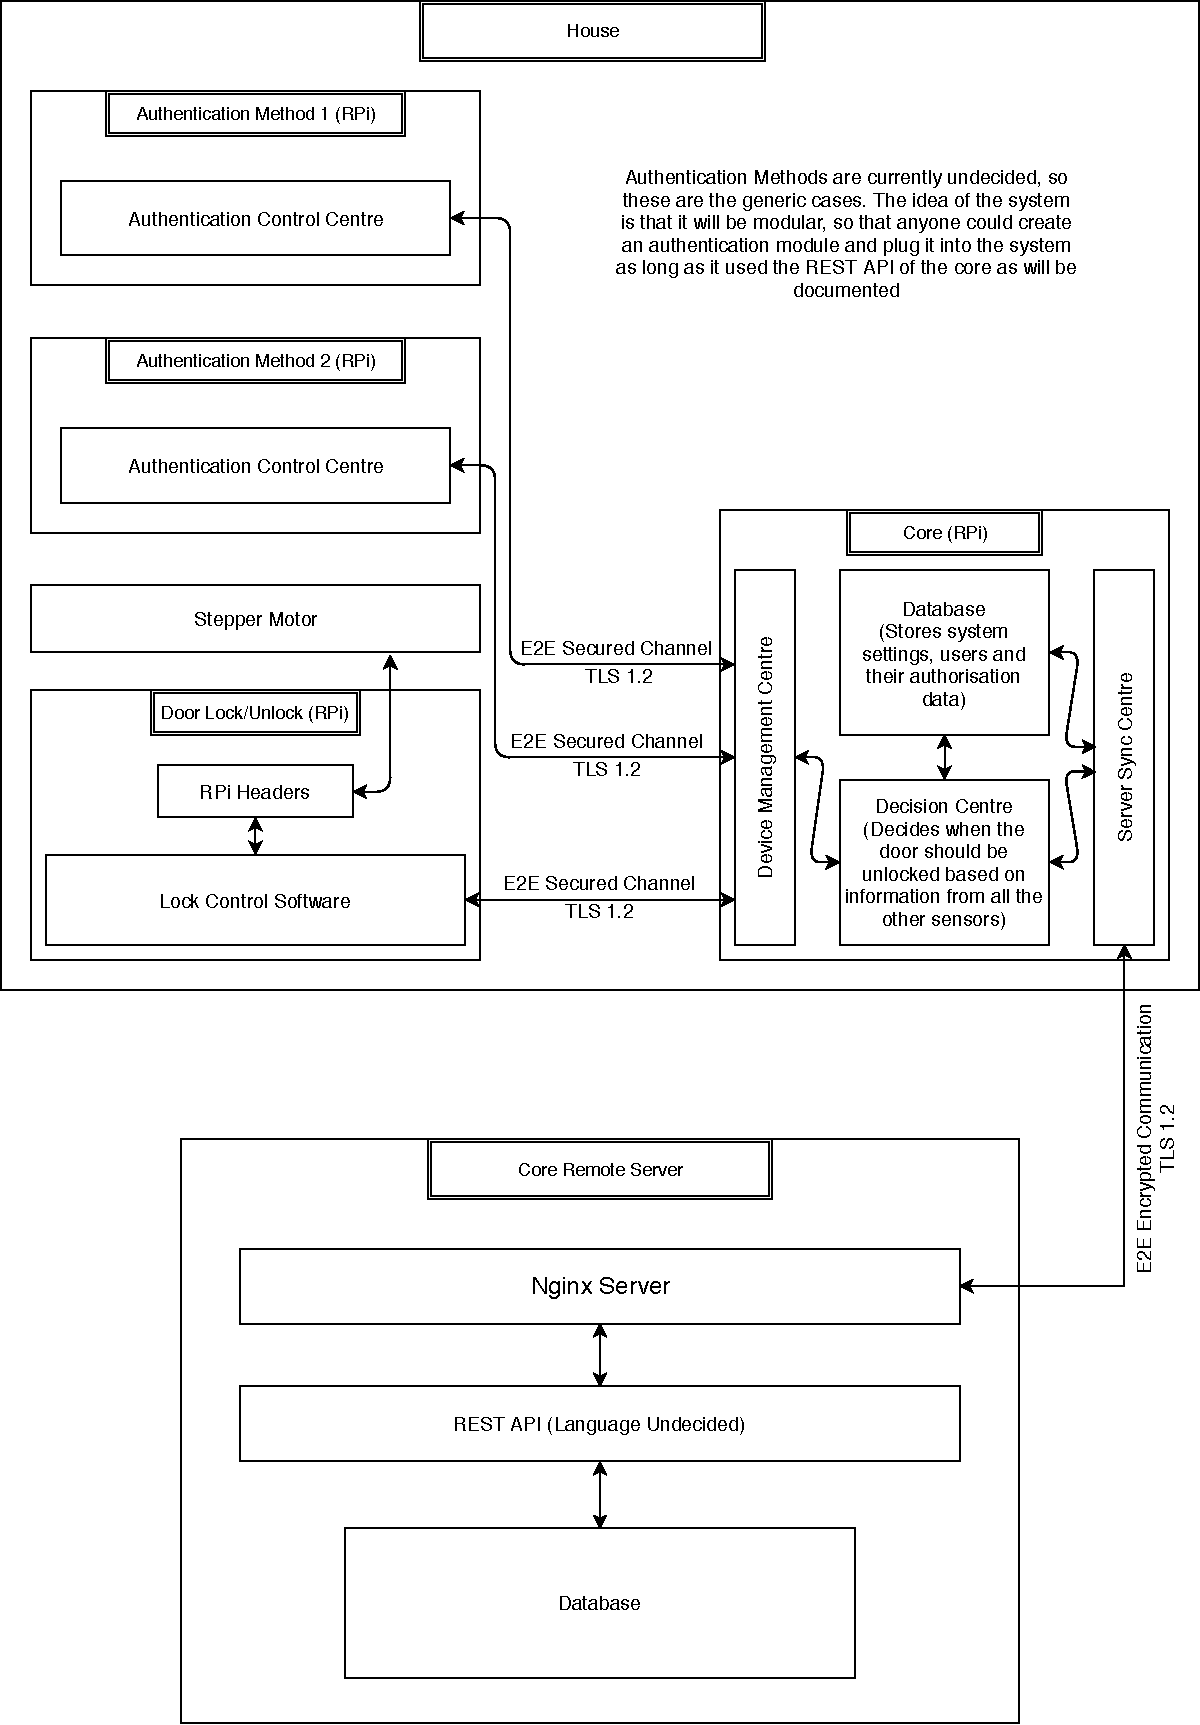
\includegraphics[height=0.6\textheight,keepaspectratio]{Graphics/FYP-Block-Diagram-Portrait}
\end{figure}

\subsection{Initial Core Raspberry Pi Setup}
Figure 4.2 below shows the planned sequence of interactions between different devices for setting up a new core raspberry pi including connecting it to the wifi and adding it to the users account. The initial setup section is mandatory, the alt section which allows the user to pair the device again at a later date is an optional implementation step and will be done if time permits.
\begin{figure}[H]
	\caption{Sequence Diagram for Setup of Core Raspberry Pi}
	\centering
		\includegraphics[height=0.6\textheight,keepaspectratio]{"Graphics/Initial Core RPi Setup"}
\end{figure}

\subsection{New Device Pairing to Existing Network}
Figure 4.3 below shows the planned sequence of interactions between different devices for setting up a new device when an existing network already exists, where a core has already been paired to an account. This process would add the new device to the existing core however this won't be needed if extra authentication methods aren't added to the network, again this will be time dependent.
\begin{figure}[H]
	\caption{Sequence Diagram for Setup of a New Device on an Existing Smart Lock Network}
	\centering
		\includegraphics[height=0.6\textheight,keepaspectratio]{"Graphics/New Device Pairing to Network"}
\end{figure}

\newpage
\section{Project Plan}
\begin{center}
	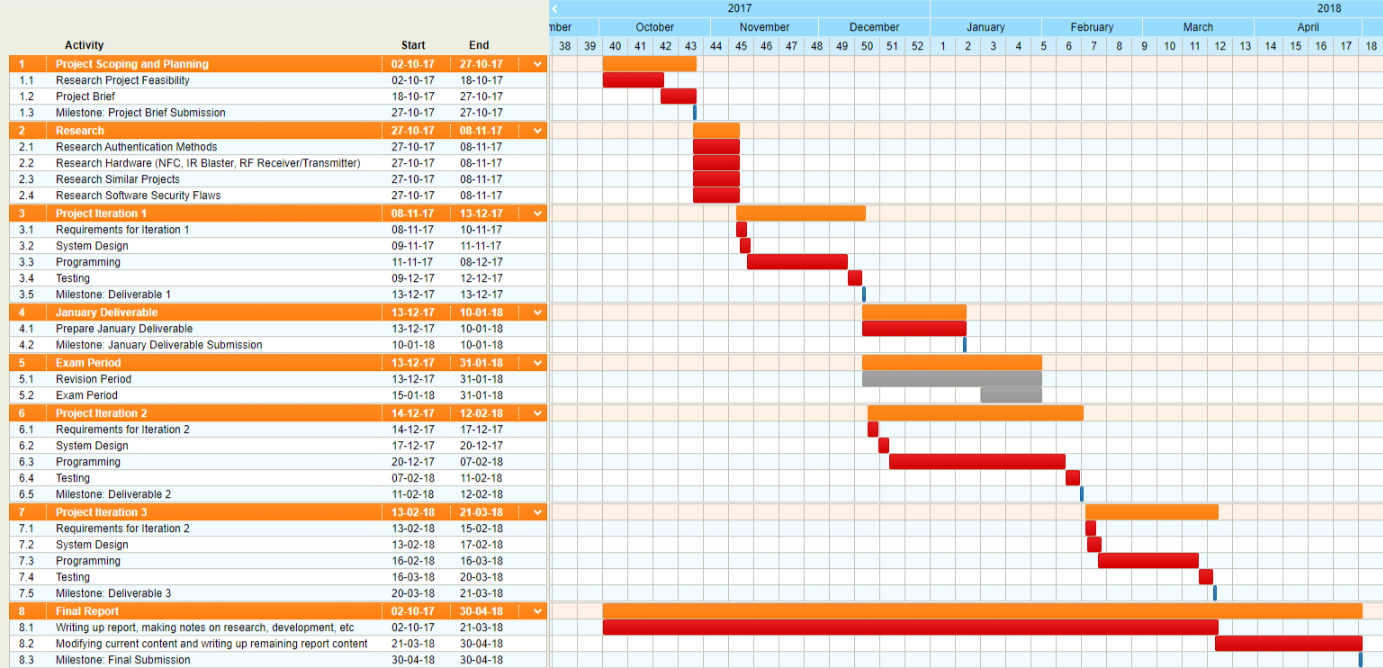
\includegraphics[angle=90,width=\textwidth,height=\textheight,keepaspectratio]{Graphics/FYP-Project-Plan}
\end{center}

\subsection{Technical Design Decisions}
In this section I will describe certain aspects of the project where I had to make decisions as to how they could be implemented best. In each section I will give a high level description of each method followed by which method I decided to go with and why. Some of the solutions may not be required as they may not get implemented in the demo, however they would be required for a full implementation and so are worth discussing.

\subsubsection{Initiate Connection from Another Device to Core Raspberry Pi}
This is a difficult issue to get around as finding a specific device on the network is not trivial, especially if the network is particularly large. There are various different ways I could solve this which are described below.

\paragraph{Method 1 - IP Broadcasting} One option is to use IP Broadcasting, where the core uses the networks broadcast range to send data to all the other devices on the network. This would work, but I'm unsure of the reliability of this method and broadcasting the IP of the core to the entire network doesn't seem like something I would want to do. It would likely be fine on a home network, however if it was on a much larger network in a business, this method may not work at all as they could block broadcasting on their switches entirely, or if multiple cores are running on the network it could become quite congested with the number of devices trying to announce themselves to other devices.

\paragraph{Method 2 - Bluetooth Sync Device to Core} This would use the Bluetooth on both devices to contact each other and find out the IP of the core on the network. The device would then use this IP to establish a connection to the core. This method has a few issues, namely the security of communicating over Bluetooth as it doesn't have the same kind of security as Wi-Fi. The other issue is that this means the two devices must be within Bluetooth range, which is much shorter than Wi-Fi range and can't be easily extended, unlike Wi-Fi range which has highly available and cheap range extenders.

\paragraph{Method 3 - Contact the remote server to get the Core IP} For this to work, the Core would have to announce its IP to the remote server whenever it changed. This would be very simple as the Core will already have a connection established to the remote server. The device that is trying to connect to the Core would then simply have to contact the remote server and request the IP of the Core on the local network, and then establish a connection with it. This is the easiest method to secure as it gives one point of contact to retrieve this information, and eliminates the need for any kind of discovery. This also allows devices to be as far away from each other as required if they are on the same network.

\paragraph{Decision}
Method 3 would be the best way to go about this as it provides the most security and is also the most simple to implement. Devices can quickly look up the IP whenever they need and have to be authorised in order to do so.

\subsubsection{Initiate Connection to Core Raspberry Pi for Initial Setup}

\paragraph{Method 1 – Connect using 4-digit code through the remote server}
The first issue here is that using a code means that you don’t have to be within proximity of the device to attach to it as it goes through the remote server to establish the link. There are some potential ways that attackers could guess or work out the code and then connect to it themselves, or find some way to force the remote server to override the owner of that Core. The initial setup should be handled on the Core itself, and the phone should not contact the remote server regarding this, the Core should contact the remote server to establish that a link has been created.

\paragraph{Method 2 – Connect using Bluetooth sync between the Core and users phone}
This method requires that the user is close to the Core to establish a link with it as they must be within Bluetooth range and push a physical button on the device to start the pairing process. If the device is already paired to an account, then it will either need to be confirmed by the current account that they want to pair to a new account or they will need to wait for a timeout to expire before the pairing can be done (unless it is cancelled from the current owners account). Within the app, they will need to select the option to connect to a new Core, and then select the Core they want to pair with from the list. The phone will then establish a Bluetooth connection with the Core, the Core will generate a private key to identify itself, and will upload the public key to the remote server for validation when communicating with it. This will bind the Core to the account the user was logged into and they will then be able to add new devices and users to the Core, as well as modify the settings for the Core, all from the app.

\paragraph{Method 3 – Connect to Wi-Fi network broadcasted by the Core on users phone}
This method requires that the used must be close to the Core to push the physical button on the device to create the Wi-Fi network to start the setup of the device. All other steps are the same as Method 2, however this method has the benefit of not requiring every device to have Bluetooth as well as Wi-Fi, lowering the physical size, cost and power required to run each device. Wi-Fi can also be more easily secured than Bluetooth, and I will carry out testing to see if I can lower the power of the Wi-Fi adapter when in access point mode to lower the range of the network, so the user must be close to the device when performing the initial setup.

\paragraph{Decision}
Method 3 is the best way to do this as we are already using Wi-Fi so don't require extra hardware on the device, also interfacing with and securing Wi-Fi is easier than Bluetooth which will save time in the development stage. 

\subsubsection{Initiate Connection from New Device to Core Raspberry Pi for Setup}

\paragraph{Method 1 – Bluetooth pairing between Device and Core}
This method would work, but could introduce difficulties for the user as it requires the two devices to be close to each other as they must be within Bluetooth range. It would also require the core to store the Wi-Fi password in a readable form to give it to new devices that will also need it. This is not something that I want to do as that means if someone can access the device then they can access the Wi-Fi password and therefore the entire network.

\paragraph{Method 2 – Bluetooth pairing between device and users phone}
This method will work in the same way as the initial setup of the core. The User will press a pairing button on the device itself, then go to an add device page on their phone (only available for people who are already admins of a Core). On this page they will see any devices that are in pairing mode that they can add to their network. Once they have added the device, the app will request they connect it to the same Wi-Fi network as the Core, and request the password for the network. The device will then have successfully been added to the door unlocking system, will exit syncing mode, and will then communicate with the Core directly. The user will see the device in their list of devices on their door unlocking system, and will be able to change any settings it has.

\paragraph{Method 3 – Wi-Fi pairing between the device and users phone}
This method will work in the same way as method 2, however it will use Wi-Fi instead of Bluetooth for the setup, for the same reasons mentioned in Method 3 of the Initiate Connection to Core Raspberry Pi for Initial Setup section.

\paragraph{Decision}
Method 3 has been chosen for the same reason as in the Initiate Connection to Core Raspberry Pi for Initial Setup section.

\subsubsection{Security During the Setup Phase}
\improvement{Write this section}